\chapter{Baseline Calibration}

\section{Framework}
%I might want to include more detail about how accurate we want it to be. Like including errors or something.

At this point in the pipeline, the positional coordinates of each antenna are only known to approximate values. Since interferometry is heavily reliant on highly accurate baseline vectors, using such rough coordinates would yield unsatisfactory visibilities. Therefore, we must calibrate our antenna baselines as a preliminary step for further data analysis. As we will explore in more detail in the following sections, the calibration process itself is performed by minimizing phase residuals between observed and predicted satellite passes. Let us first visualize what our antenna array might look like with an example shown in Figure~\ref{fig:ant_cluster}.

\begin{figure}[H]
  \centering
  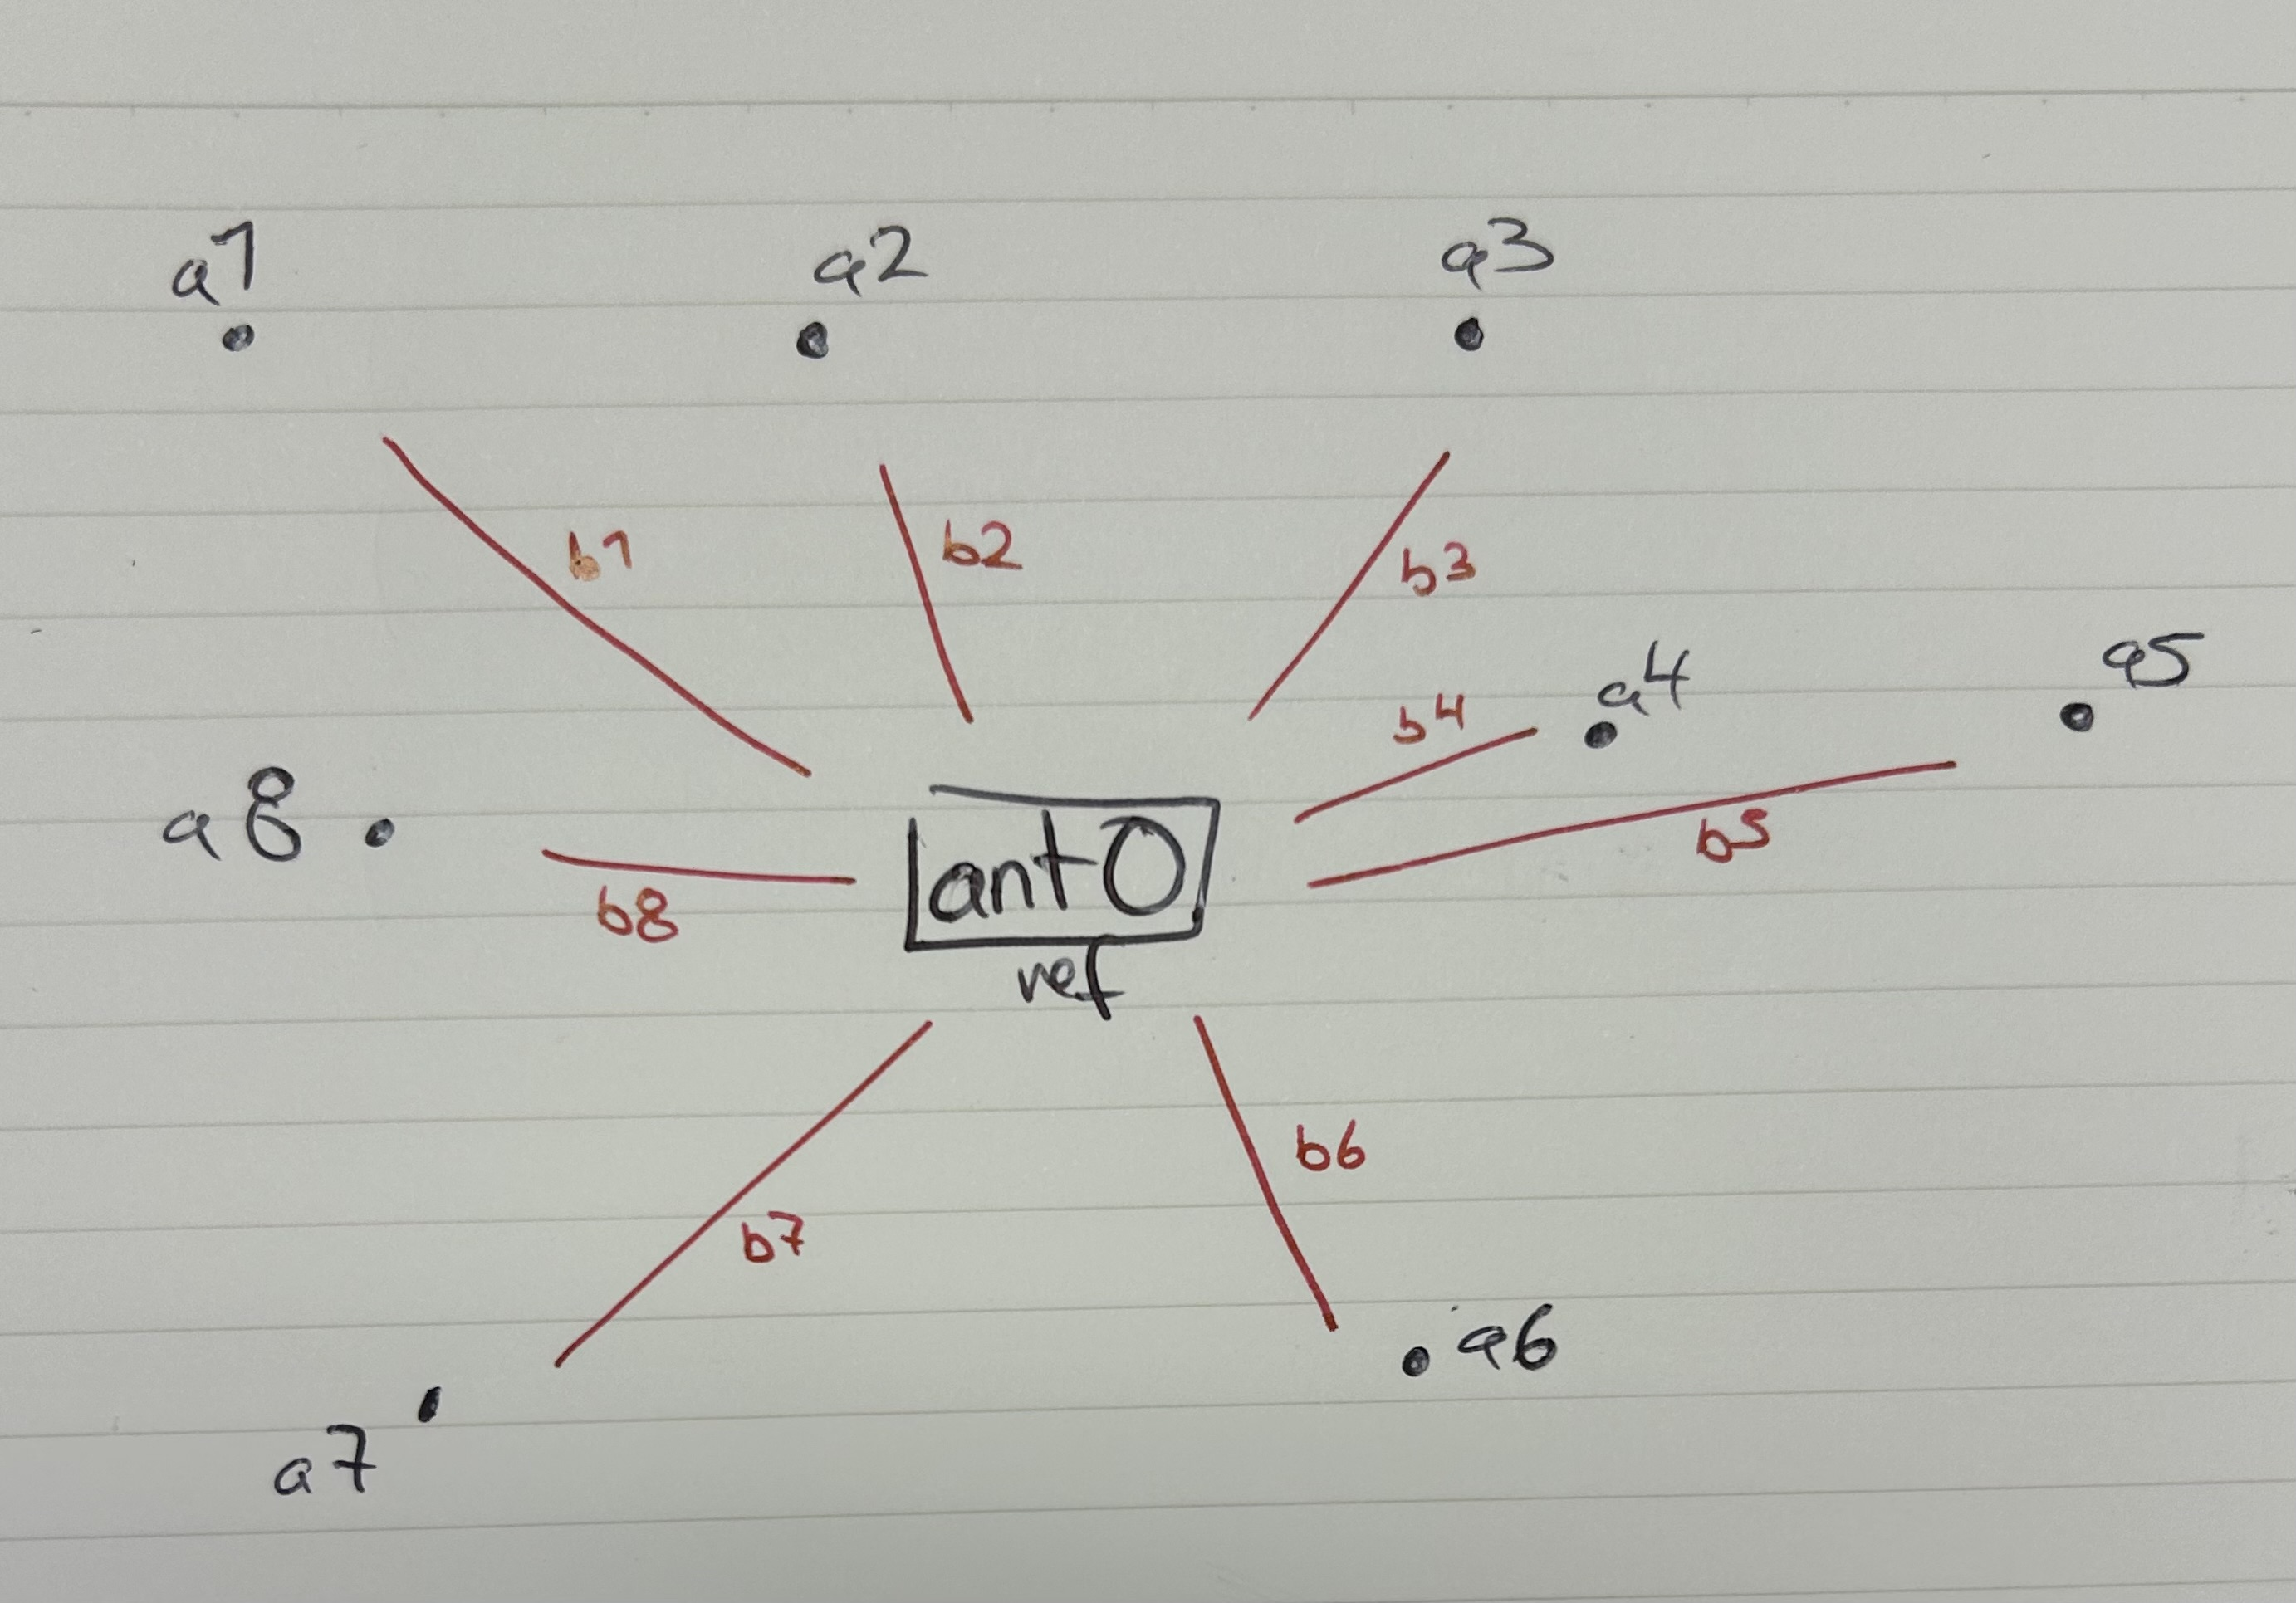
\includegraphics[width=0.5\linewidth]
  {Figures/baseline_array_placeholder.jpg}
  \caption{Example of Antenna Cluster. Reference Antenna need not be centrally positioned.}
  \label{fig:ant_cluster}
\end{figure}

We initially define a reference antenna (also referred to as Antenna 0), which will keep its initial estimated coordinates 
throughout the fitting. 
All other antenna are labeled with natural numbers 1, 2, 3, and so on. 
We only consider baselines originating from the reference antenna, and label them by the name of their connecting non-reference antenna. 
For example, as seen in Figure~\ref{fig:ant_cluster}, the baseline connecting Antenna 0 to Antenna 5 is labeled baseline 5.

Since we only require baseline vectors and not actual geodetic coordinates, a highly precise antenna position with respect to earth is 
of secondary importance. 
This allows us to fit each of these baselines individually and independently, using the non-reference coordinates as the only fitting parameter, 
determining the value which returns the best relative coordinates. 

With the general layout in mind, we observe the overall Baseline Calibration data flow in Figure~\ref{fig:flow}.

\begin{figure}[H]
    \centering
    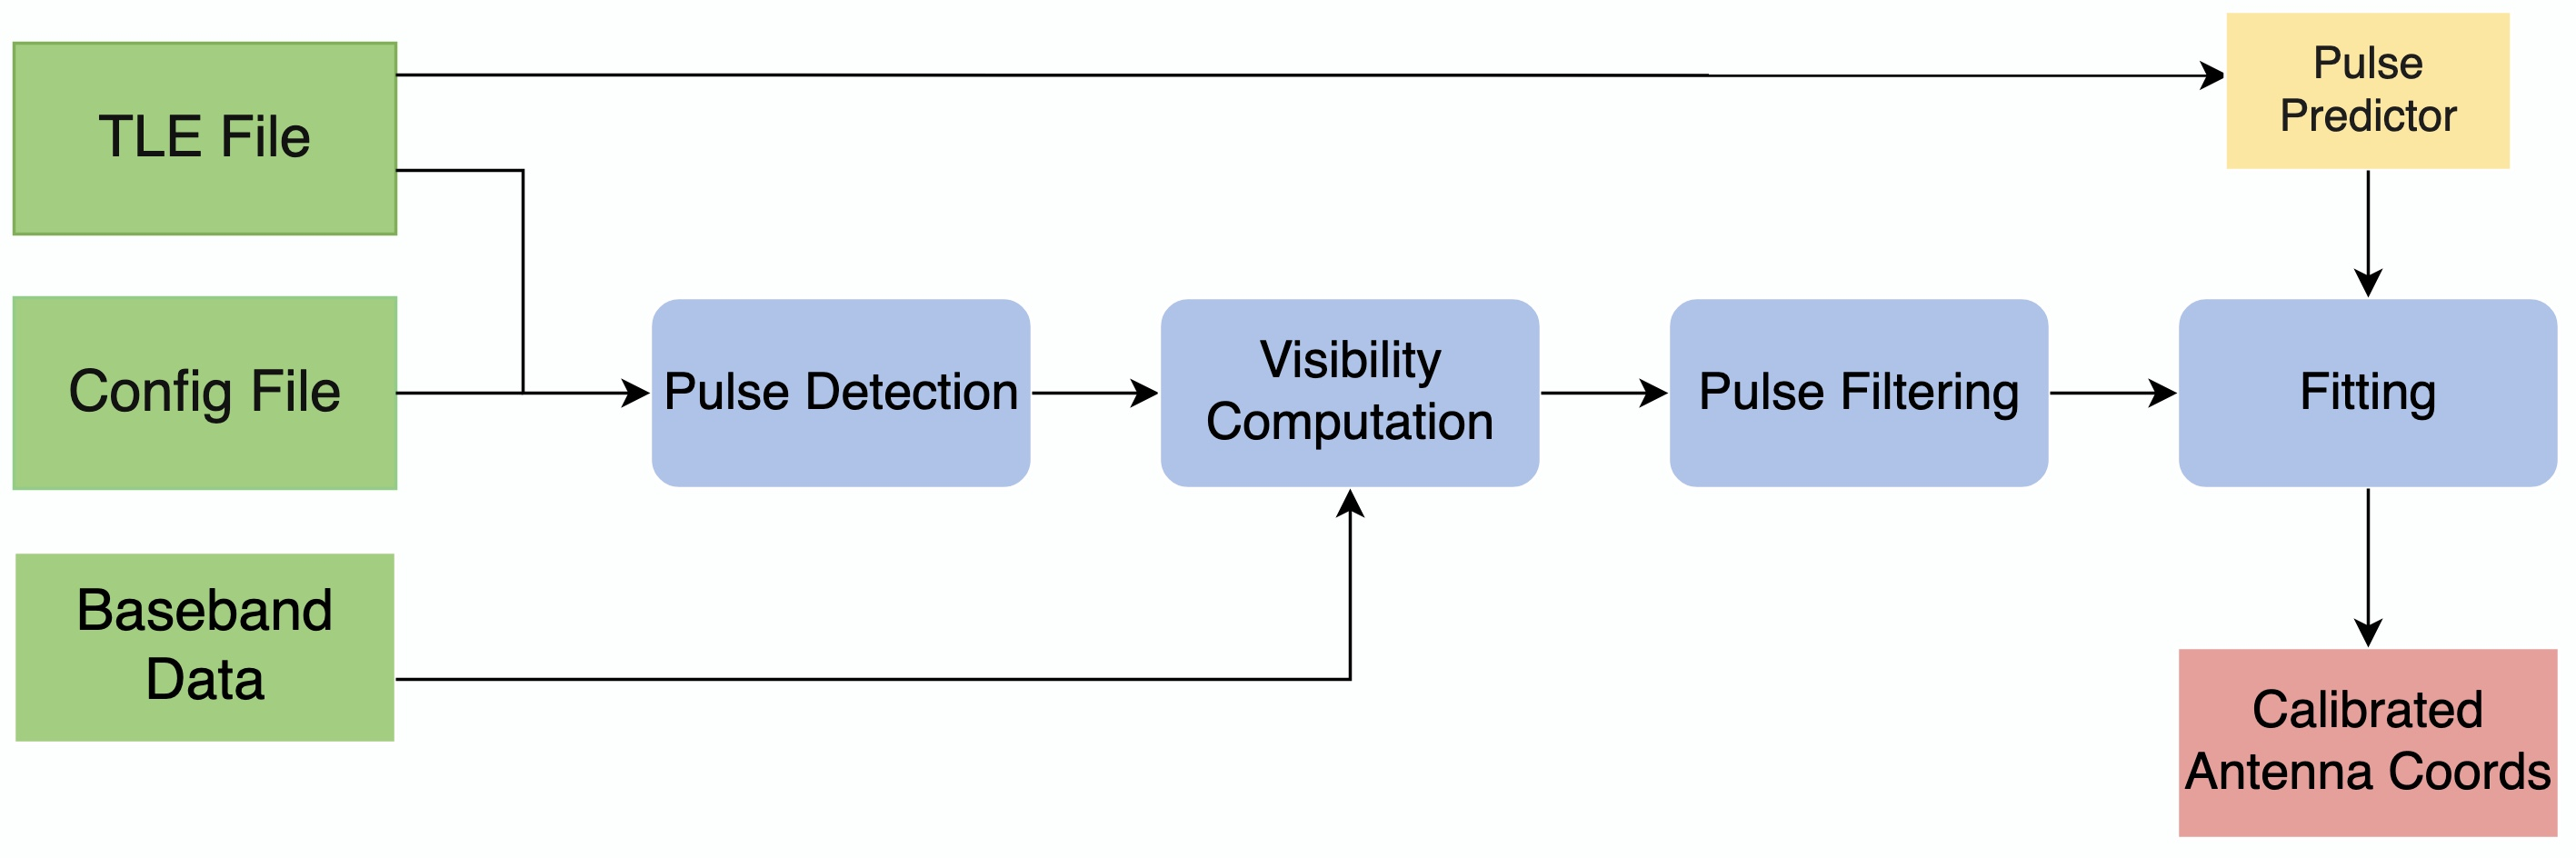
\includegraphics[width=\linewidth]{Figures/flowchart.jpeg}
    \caption{The Data flow is split into four main working modules (blue), 
    with three primary inputs (green), one fitting predictor function (yellow), and one primary output (red).}
    \label{fig:flow}
\end{figure}

Visibility Computation and filtering, the main observed data processing, are detailed in Section~\ref{sec:observed}. 
Phase prediction and synthesis is discussed in Section~\ref{sec:predicted}. 
Finally, the fitting process and its complications is outlined in Section~\ref{sec:fitting}. 
Since this process is still in development, we explain the future outlook in Section~\ref{sec:future}.

\section{Observed Pulses}
\label{sec:observed}

\subsection{Theoretical Pulse}

Let us again consider a single two-dimensional satellite pulse (shown previously in Figure~\ref{fig:sat_pulse}). 
We make assumptions of a flat sky, high satellite signal brightness, and uniform antenna response to simplify the theory.
Recall that we performed a cross cross correlation and found the exact spectrum number offset. 
Thus, using the raw baseband data, if we correct for known clock offset $\tau_c$ and perform direct cross correlation,
we will obtain complex visibilities with the geometric time delay $\tau_g$ encoded into them. This is derived below, using an integration time of $t_{\text{int}}$:
\begin{eqnarray}
    V_{0,1} &=& \int^{t_0 + t_{\text{int}}}_{t_0}  E_0(t) E_1^*(t) dt, \\\nonumber
    &=&  \int^{t_0 + t_{\text{int}}}_{t_0} E_0(t) \left[ E_0 (t) e^{2 \pi i \nu_0 \tau_g(t)} \right]^* dt,  \\\nonumber
    &=&  \int^{t_0 + t_{\text{int}}}_{t_0} E_0(t) E_0^*(t) e^{-2 \pi i \nu_0 \tau_g} dt, \\\nonumber
    &=&  e^{-2 \pi i \nu_0 \tau_g} \int^{t_0 + t_{\text{int}}}_{t_0} |E_0(t)|^2  dt
\end{eqnarray}
Here we assume that the satellite moves slowly with respect to the integration time, which allows us to extract the phase from the integral.
Therefore, we consider $\tau_g(t)$ to be constant for a single visibility computation. 
Thus, we have a complex visibility which has the geometric delay encoded into it, 
so for many pulses we can unwrap this phase and obtain a phase plot over time.
Moreover, even when not purely narrowband, we still expect a dominant presence of the $e^{-2 \pi i \nu_0 \tau_g}$ term as $E_0$ 
correlated with itself is very large.




\subsection{Practical Pulse}

Practically, we compute visibilities per chunk, blah blah

We use an accumulation length of $3*10^5$ spectra, with each spectrum having a period of approximately $16 \mu s$, 
leaving us with a chunk period of approximately $0.5s$. 
Usable sections of pulses usually last several minutes, meaning they typically contain between 500 and 1000 chunks.
i here is the index in the spectrum number, N is the accumulation length, i.e. length of chunk. 
\begin{eqnarray}
    V_{0,1,i} &=& \frac{1}{N} \sum_{i = 0} ^ {N-1} E_0[i]E_1[i] \\\nonumber
    &=& \frac{1}{N} \sum_{i = 0} ^ {N-1} \left| E_0[i] \right|^2 e^{2 \pi i \tau_g[i]}
\end{eqnarray}


Figure~\ref{fig:wrapped_phase} shows the angle with time for the visibility of all channels during a pulse. 
Can clearly see how the angle of the geometric time delay dominates channels index 2 and 3. 
 
\begin{figure}[H]
  \centering
  \begin{minipage}{0.45\textwidth}
    \centering
    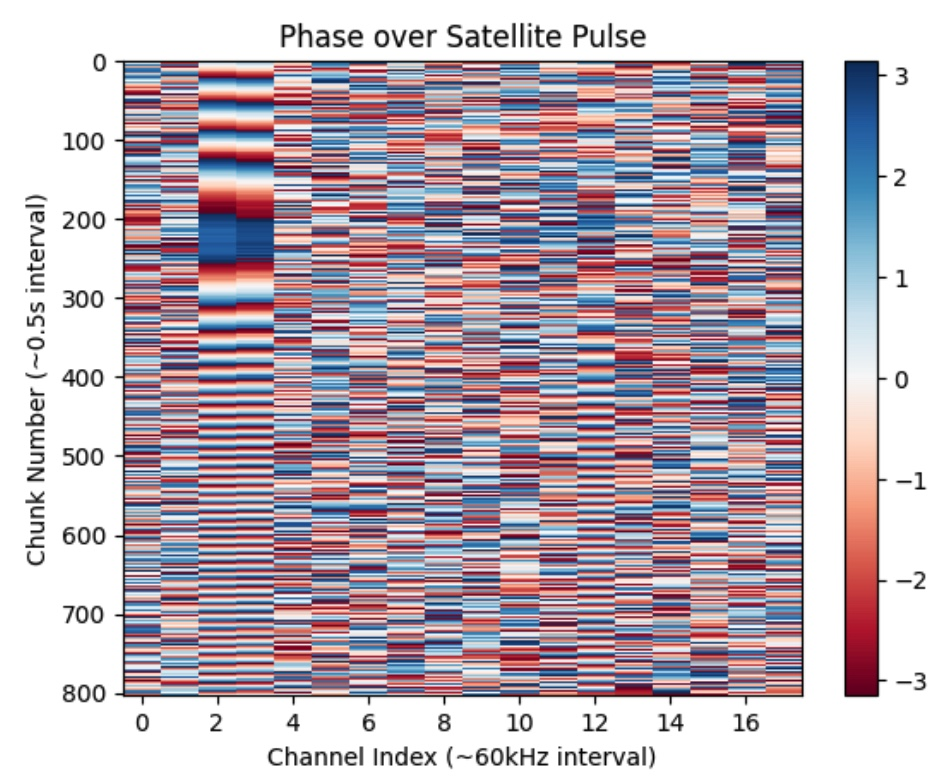
\includegraphics[width=\linewidth]{Figures/wrapped_phase_example.jpeg}
    \caption{Wrapped visibility phase. The satellite pulse is visible in channels 2 and 3.}
    \label{fig:wrapped_phase}
  \end{minipage}
  \hfill
  \begin{minipage}{0.45\textwidth}
    \centering
    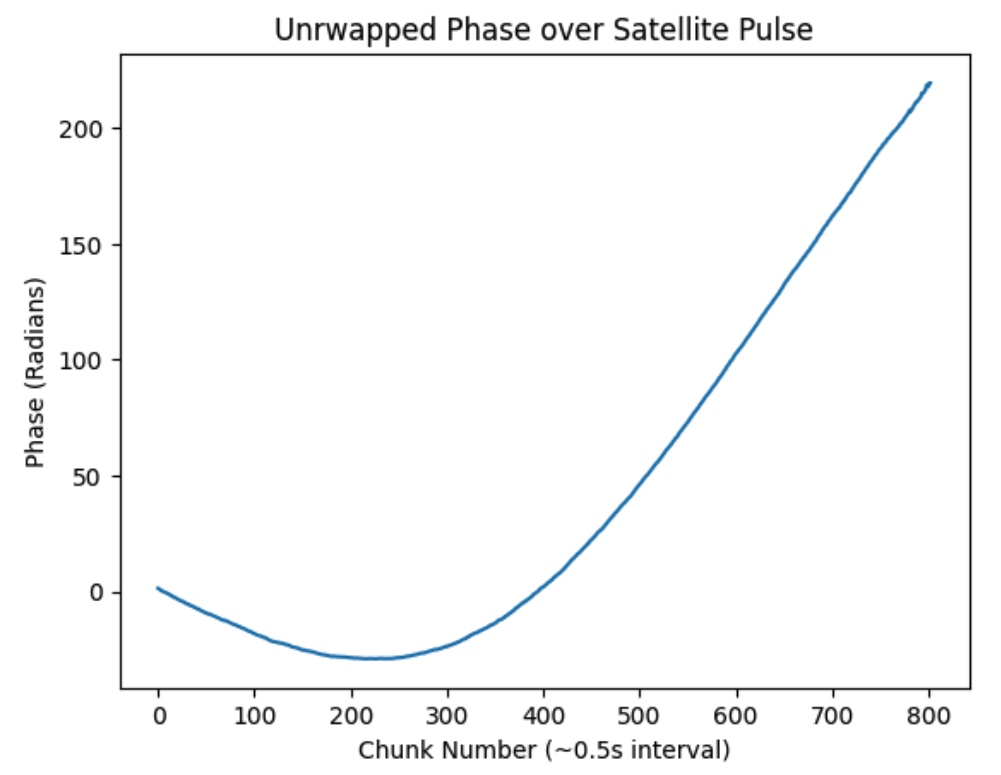
\includegraphics[width=\linewidth]{Figures/unwrapped_phase_example.jpeg}
    \caption{Unwrapped phase for channel 2 over the entire pulse.}
    \label{fig:unwrapped_phase}
  \end{minipage}
\end{figure}


To obtain the observed phase for each satellite pulse, we must use the satellite detection script 
(outlined in Chapter~\ref{chap: timing}) to get the pulse times, channels, and the spectrum number offsets. 
Spectrum number, of course, being our proxy for time. 
We correct for this as our clock offset $\tau_c$. 
Once this information is recorded and implemented, we can correlate Baseband data from the reference 
and non-reference antenna to obtain raw visibilities. We do this for each pulse, for each day of data, and for each baseline.


The unwrapped phase is the final product of the visibility computation, and will be used as our observed data 
for the eventual coordinate fit. 
For each baseline, the total observed data is compromised of several such unwrapped pulse phase curves. 


\subsection{Filtering}

Oftentimes, the visibility will be rather messy.
The pulse filtering process ensures we obtain a continuous, reasonably smooth phase plot.
It involves the following steps:

\begin{enumerate}
  \item There is often missing data in the 1bit visibilities, due to a lack of data in the chunk. We interpolate over the complex data
        directly to ensure the visibility is continuous.
  \item When unwrapping the phase, there are some parts of the pulse that have almost no distinguishable phase, and must be cut out.
  \item Finally, in the good portions of the phase, there can be jagged jumps, which are interpolated over smoothly (in visibility?). 
        this is either caused by bad data or by aliasing (since the satellite phase angle can change very fast).
\end{enumerate}

For the time being, this is all conducted manually. 
The aim is to automate this process to improve reproducability and speed.



\section{Predicted Phase}
\label{sec:predicted}

In order to correctly fit the non-reference antenna's coordinates, we must construct a function which 
accurately predicts the satellite pulse phase over time. 
Its only free parameter must be the non-reference antenna's coordinates. 
Once we have constructed this function, we can evaluate the \textit{goodness of fit} of the initial guess coordinates as a preliminary test. 
This can be seen in Figure~\ref{fig:unfitted}.


\begin{figure}[H]
  \centering
  \begin{minipage}{0.45\textwidth}
    \centering
    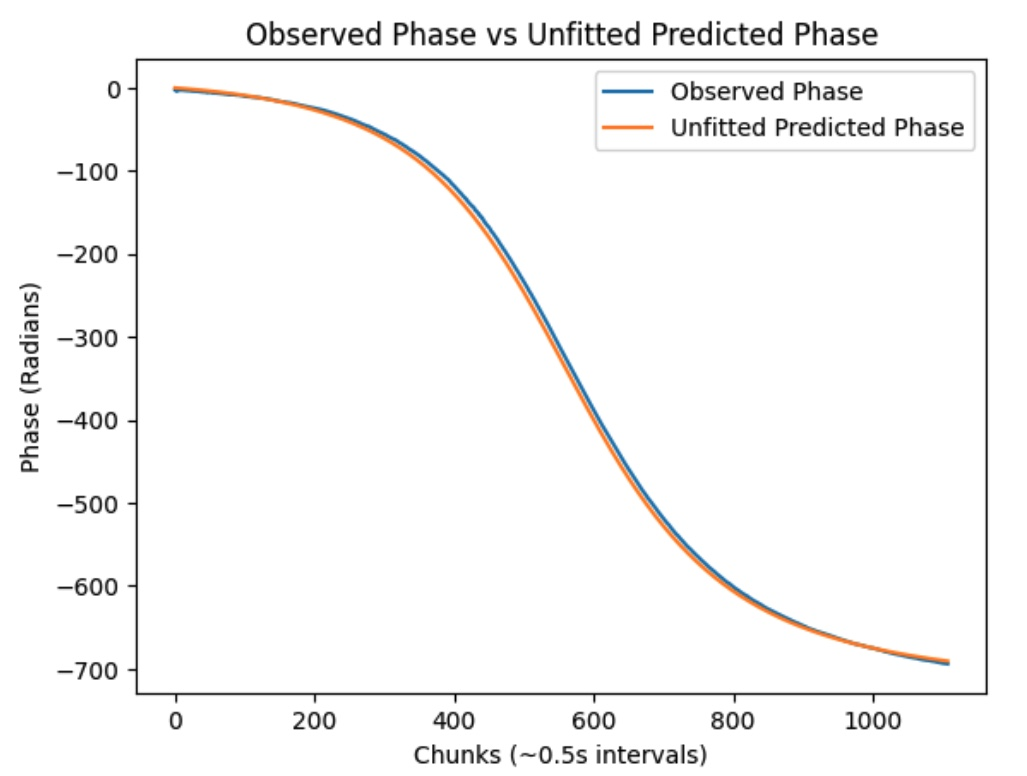
\includegraphics[width=\linewidth]{Figures/observed_vs_unfitted_predicted_phase.jpeg}
  \end{minipage}
  \hfill
  \begin{minipage}{0.45\textwidth}
    \centering
    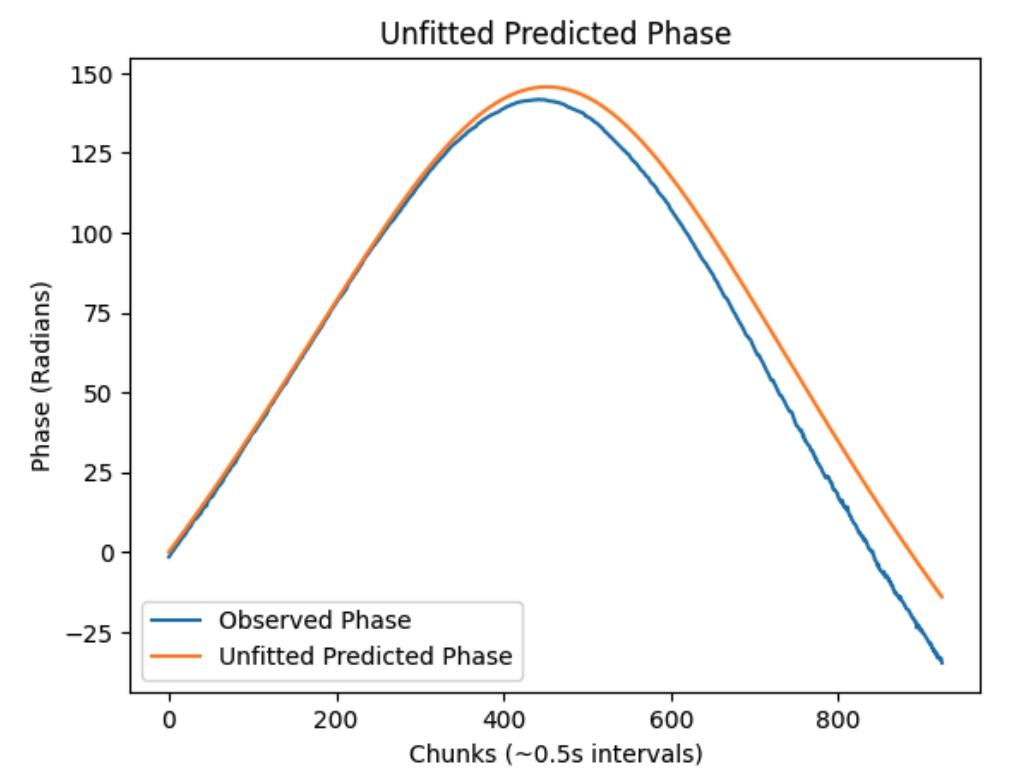
\includegraphics[width=\linewidth]{Figures/obs_vs_unfitted_pred_2.jpeg}
  \end{minipage}
  \caption{Two examples of unfitted predicted phases against their observed counterparts.}
  \label{fig:unfitted}
\end{figure}

Figure~\ref{fig:unfitted} illustrates the necessity of fitting for multiple satellite passes simultaneously, 
as different satellites will have different trajectories in the sky, and thus will favor different fits.





\section{Fitting}
\label{sec:fitting}

%notes to add

% - question of directionality
% - 

\subsection{Moving Parts}

There are several things we need to take into account during the fitting process. 

First of all, we must take into account the thermal noise on each pulse. The residuals of each pulse must be weighted using the noise of the pulse, to ensure that noisy pulses are considered less.

Secondly, we must ensure that our various pulses cover several different directions in the sky. A baseline is a single line, so passes have to move over at different angles to properly calibrate it. DEVELOP?


\begin{figure}[H]
    \centering
    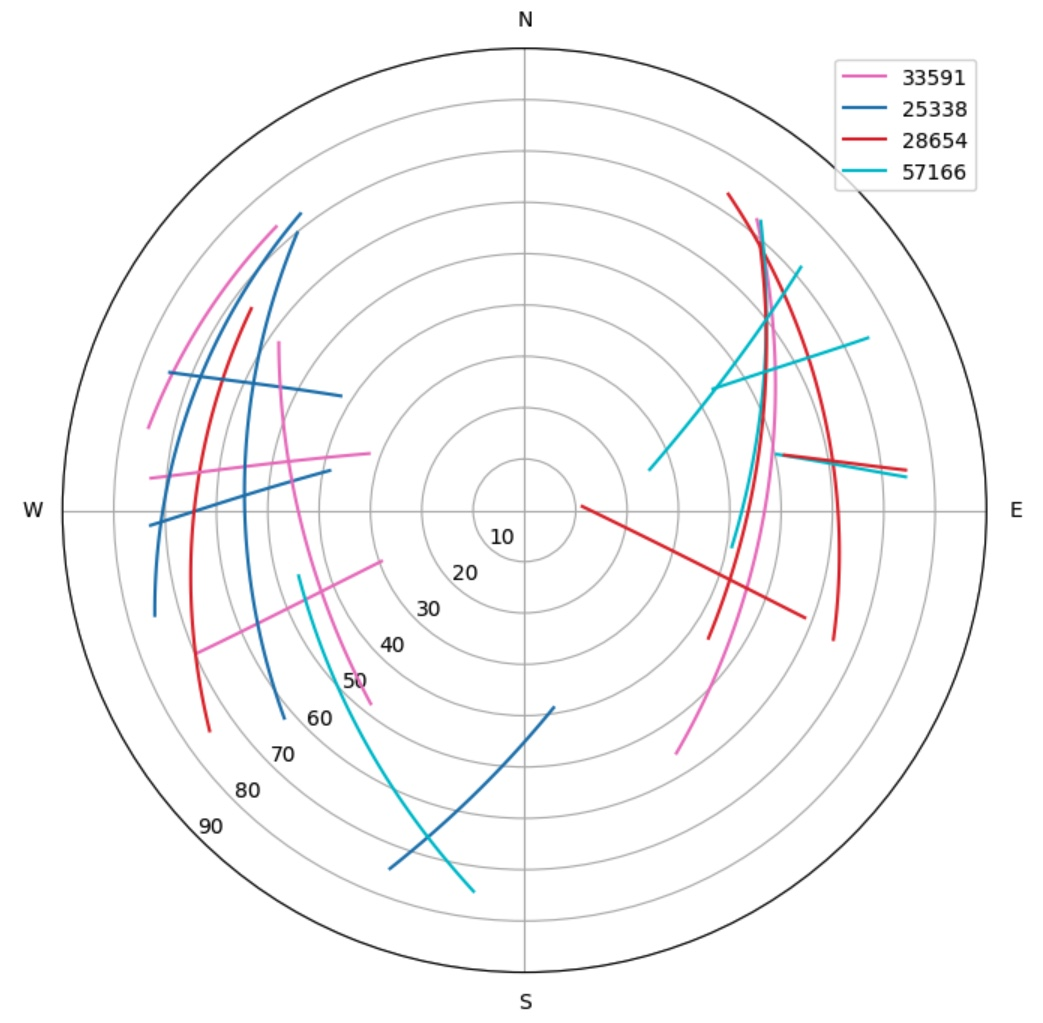
\includegraphics[width=0.4\linewidth]{Figures/satpass_plot.jpeg}
    \caption{Example of a satellite pulse plot, in direction over the sky}
    \label{fig:satpulse_plot}
\end{figure}


Finally, we must take into account offset between predicted phases and observed phases. We assume that when we predict a phase, it is accurate in human observer time. We also assume (and pray) that the visibility spectrum number offset correctly aligns the two clocks of the two antenna. This is done in such a way that leaves Antenna 0's clock unchanged, and shifts the spectra of Antenna 1 (which makes sense or else it would be super confusing with multiple antenna). But we know that there is significant clock drift in the human time (RPI) clock of the Antenna. Since each pulse is accessed separately using human time, each pulse has the risk of having a time offset associated to it. So we must implement a per-pulse time offset variable that can correct for this. 

Therefore, the fitting process has three separate weighting methods, alongside three separate fitting types. These are modular; any fitting method can be used with any of the weighting methods. 



\subsection{Weighting Methods}


\subsection{Fitting Methods}

We do several types of fits. First is only with coordinates.

Obtain residuals from each pulse, concatenate into one large array, and least squares fit with your predictor function. Only fitting parameter is the coordinate for the predicted phase. This is done simultaneously for all considered pulses.

This gives us one possible fit for one baseline. 


%lowkey here you don't have to spam a bunch of plots
Figure~\ref{fig:obs_vs_fitted_all} shows six pulses with their fitted phases. 

\begin{figure}[H]
    \centering
    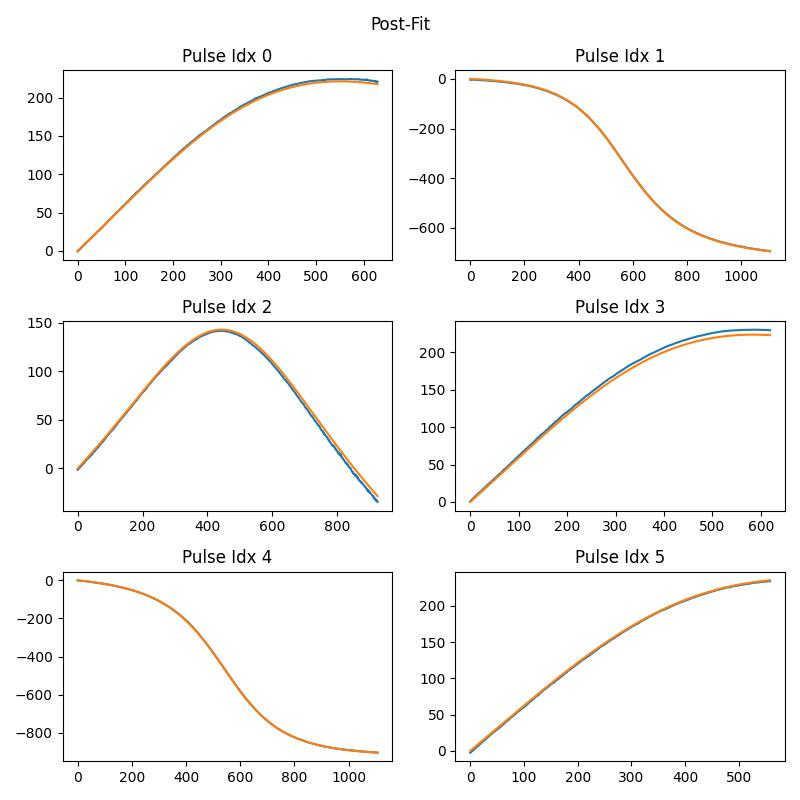
\includegraphics[width=0.7\linewidth]{Figures/post_fit_calib_plots_tlm_1721900002.jpg}
    \caption{Fitted with the TRF method. In this run, TRF and LM gave negligibly different results.}
    \label{fig:obs_vs_fitted_all}
\end{figure}

We can see how Pulse Index 1 (seen unfitted in Figure~\ref{fig:obs_vs_unfitted}) has very close agreement between observed and predicted phases. This is further exemplified in the residuals plots, seen in Figure~\ref{fig:resids_all}.

\begin{figure}[H]
    \centering
    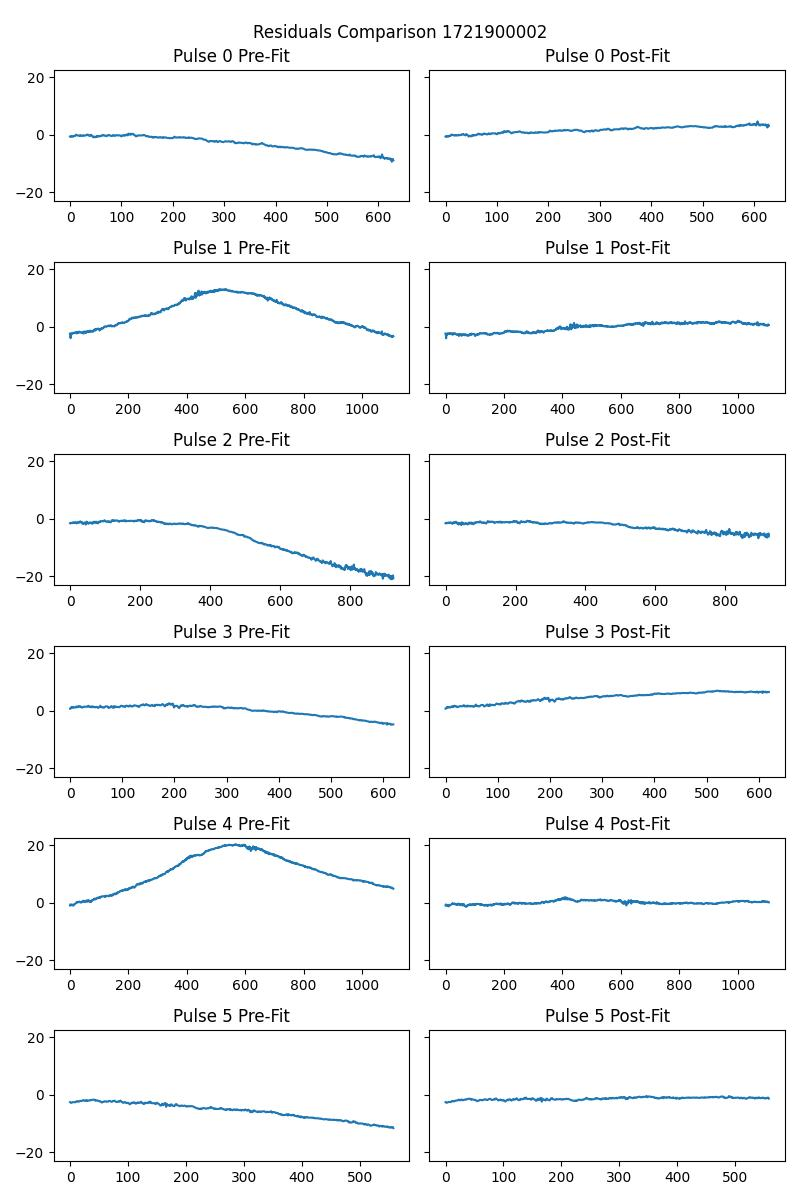
\includegraphics[width=0.5\linewidth]{Figures/residuals_individual_tlm_coordfit_1721900002.jpg}
    \caption{All pulses with residuals before and after fitting. Again with TRF algorithm.}
    \label{fig:resids_all}
\end{figure}


Secondly, we have a per-pulse time offset fit. The reason for this is the time discrepancy (in human observer time) between getting 


\subsection{Testing Methods}

To ensure we have found a valid coordinate, we must conduct some testing. Naturally, this means varying some fixed parameters and ensuring our coordinates converge to the same values. 

First, we must vary the initial guess for the non-reference antenna. This ensures that the fit is not stuck in a local minimum. In testing, several randomly generated nearby coordinates are also tested, and their results are compared. For a coordinate to be deemed valid, they must all return negligible differences in coordinates.

Second, we utilize two fitting methods as a safety check. We use both the 'Trust Region Reflective' and 'Levenberg-Marquardt' algorithms of least squared fitting. For a coordinate to be deemed valid, both fit method must yield a negligible differences. 

Third, we fit over multiple sets of 5-6 pulses, and vary combination of satellites. This ensures there is no bias in pulse direction, satellite type, or time of day. A valid coordinate must, as for other variables, remain consistent across pulses.

These tests are conducted for each baseline, using the single baseline coordinate calibration script.




\section{Limitations and Future Development}
\label{sec:future}

As of the writing of this section, there are several technical limitations causing difficulties in the development of a streamlined, generalized coordinate calibration script.

The main issue is the inconsistency in observed phase plots. This is the result of low SNR satellite passes (which are detected but not good), unwrapping bugs, or missing data. This means pulses must be combed through manually before being passed through the calibration script, significantly slowing analysis. Figures~\ref{fig:bad_pulse_phase1} and ~\ref{bad_pulse_phase2} provide an example of such a pulse.

This issue will be resolved before making a generalized script that can fit and test coordinates multiple baselines automatically. This would be the optimal case, and would significantly facilitate any future project's baseline optimization.


